\documentclass[border=15pt, tikz, multi=tikzpicture]{standalone}
\usepackage{amssymb}  % \checkmark
\usetikzlibrary{positioning, arrows.meta, fit, backgrounds, calc}

% Code-reference text style — used inline in TikZ node bodies.
\newcommand{\code}[1]{{\scriptsize\ttfamily\color{black!50}#1}}

\begin{document}

% ─── Figure 1: Trust establishment timeline (operators + admission) ─────────
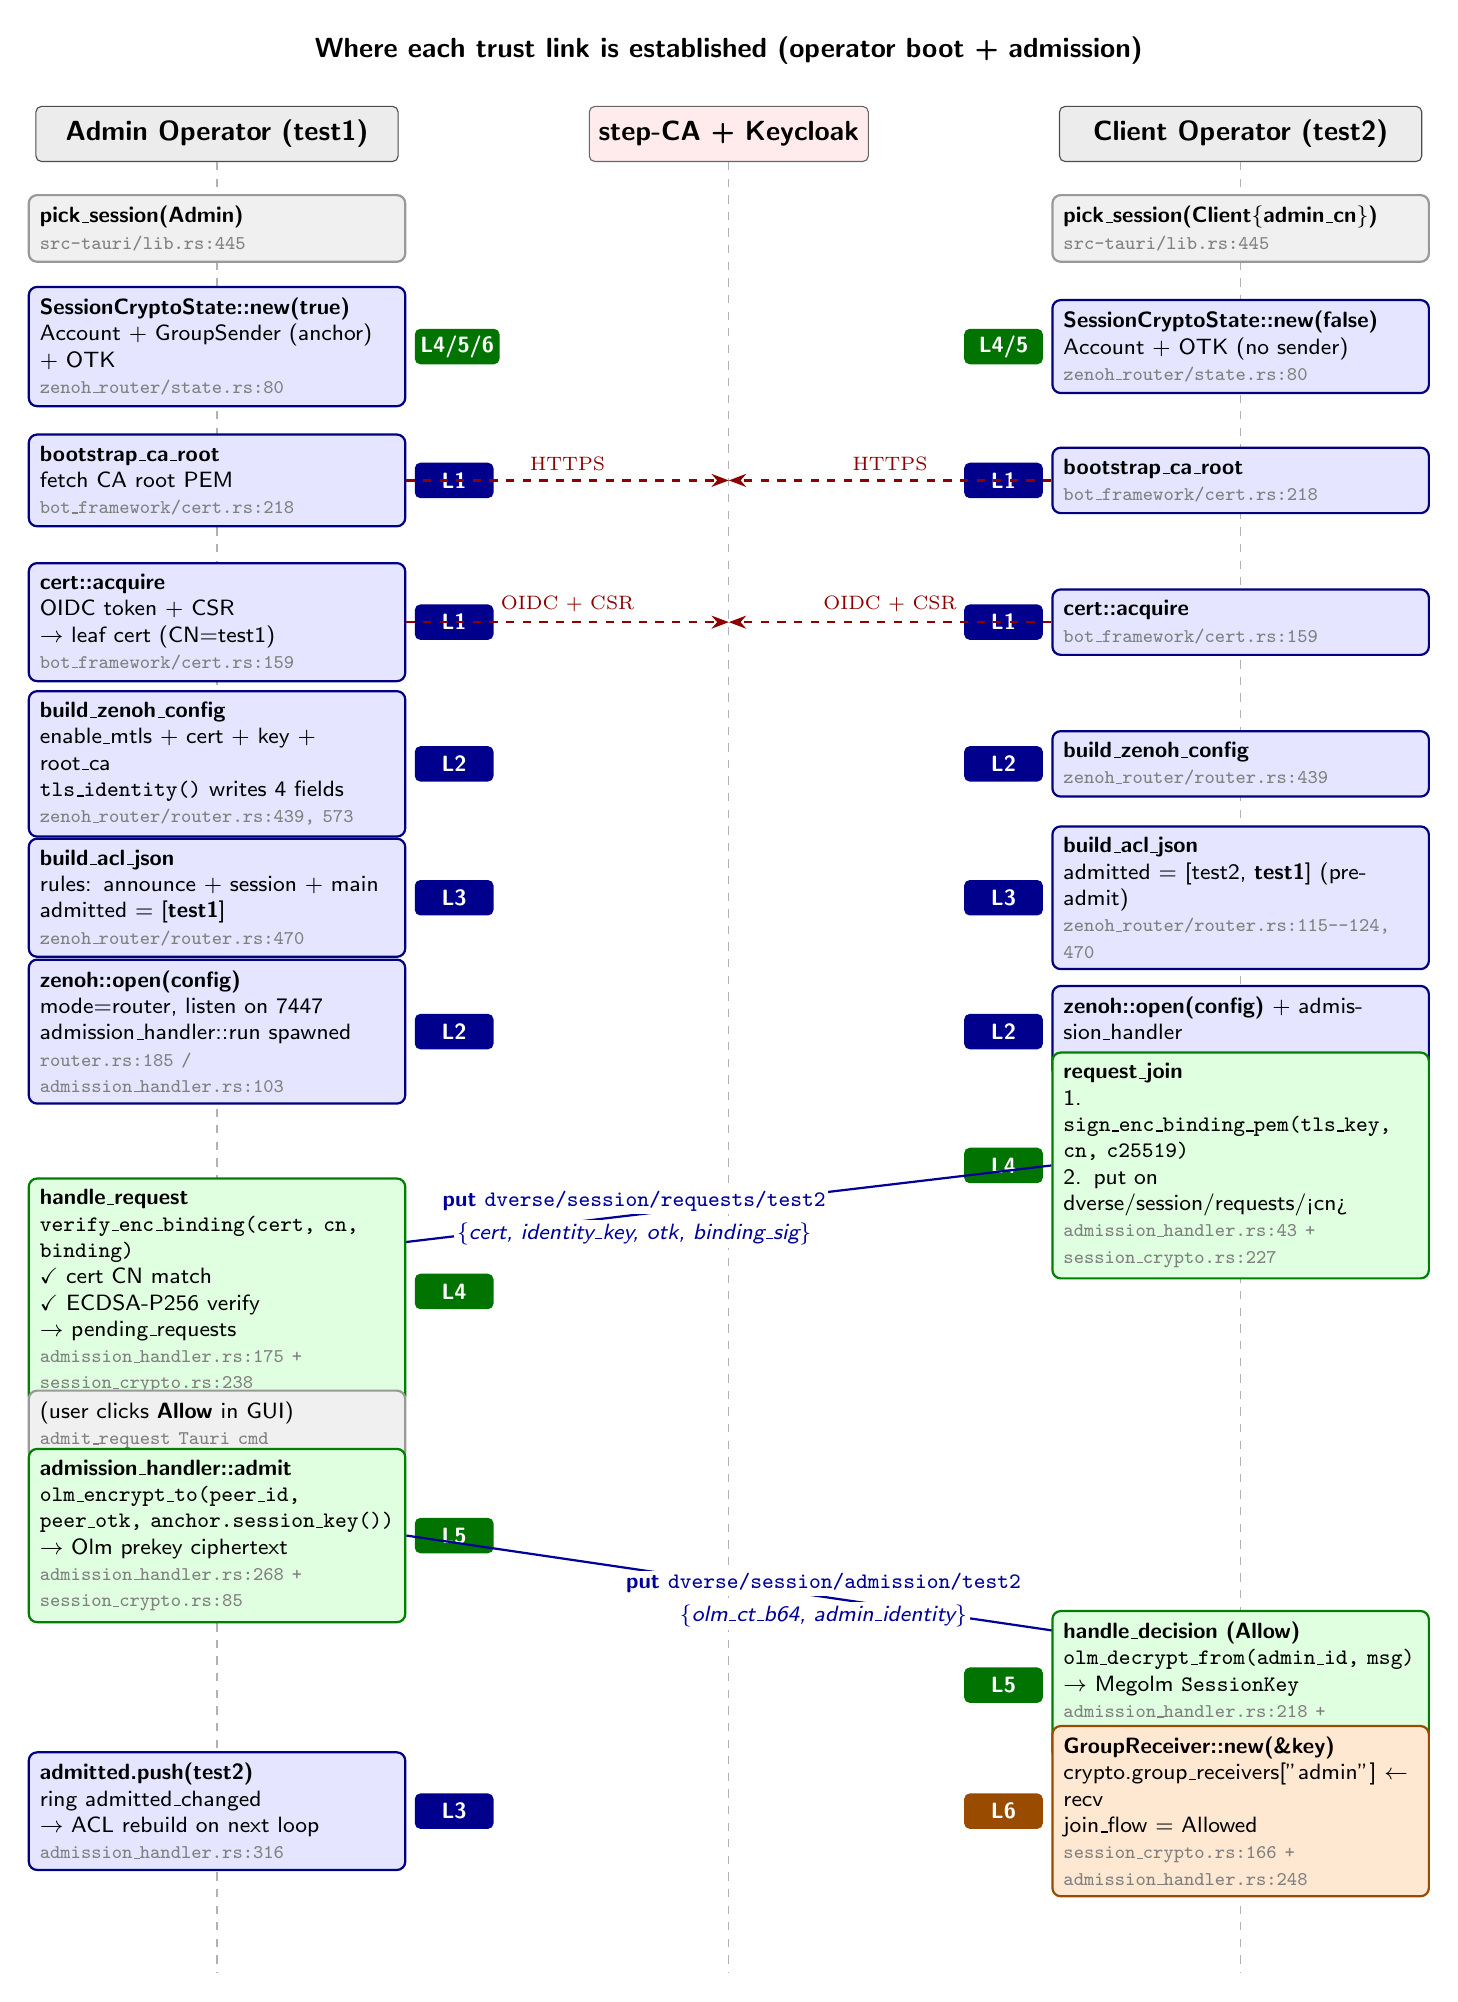
\begin{tikzpicture}[
    actor/.style={
      font=\sffamily\bfseries, align=center,
      draw=black!70, fill=gray!15, rectangle, rounded corners=2pt,
      minimum width=4.6cm, minimum height=0.7cm,
    },
    extactor/.style={
      font=\sffamily\bfseries, align=center,
      draw=black!60, fill=red!8, rectangle, rounded corners=2pt,
      minimum width=3.2cm, minimum height=0.7cm,
    },
    fabric/.style={
      font=\footnotesize\sffamily, align=left,
      fill=blue!10, draw=blue!50!black, thick,
      rectangle, rounded corners=3pt, inner sep=4pt,
      text width=4.5cm,
    },
    session/.style={
      font=\footnotesize\sffamily, align=left,
      fill=green!12, draw=green!50!black, thick,
      rectangle, rounded corners=3pt, inner sep=4pt,
      text width=4.5cm,
    },
    payload/.style={
      font=\footnotesize\sffamily, align=left,
      fill=orange!18, draw=orange!60!black, thick,
      rectangle, rounded corners=3pt, inner sep=4pt,
      text width=4.5cm,
    },
    bootstrap/.style={
      font=\footnotesize\sffamily, align=left,
      fill=gray!12, draw=black!40, thick,
      rectangle, rounded corners=3pt, inner sep=4pt,
      text width=4.5cm,
    },
    tag/.style={
      font=\footnotesize\sffamily\bfseries, text=white,
      draw=none, rectangle, rounded corners=2pt,
      minimum width=1.0cm, minimum height=0.45cm,
      inner sep=2pt,
    },
    L1/.style={tag, fill=blue!55!black},
    L2/.style={tag, fill=blue!55!black},
    L3/.style={tag, fill=blue!55!black},
    L4/.style={tag, fill=green!45!black},
    L5/.style={tag, fill=green!45!black},
    L6/.style={tag, fill=orange!60!black},
    msg/.style={-{Stealth[length=2.5mm]}, thick, blue!60!black},
    extmsg/.style={-{Stealth[length=2.2mm]}, thick, red!55!black, dashed},
    msglabel/.style={
      font=\footnotesize\sffamily\bfseries, midway, above,
      fill=white, inner sep=1pt,
    },
    msgpayload/.style={
      font=\footnotesize\sffamily\itshape, midway, below=0.5mm,
      fill=white, inner sep=1pt,
    },
    life/.style={dashed, gray!60},
]

% ── Actors ──
\node[actor]    (Adm) at (0, 0)   {Admin Operator (test1)};
\node[extactor] (X)   at (6.5, 0) {step-CA + Keycloak};
\node[actor]    (Cli) at (13, 0)  {Client Operator (test2)};

% ── Lifelines ──
\draw[life] (Adm.south) -- ++(0, -23);
\draw[life] (X.south)   -- ++(0, -23);
\draw[life] (Cli.south) -- ++(0, -23);

% ── Bootstrap row ──
\node[bootstrap, anchor=center] at (Adm |- 0, -1.2)
  {\textbf{pick\_session(Admin)}\\\code{src-tauri/lib.rs:445}};
\node[bootstrap, anchor=center] at (Cli |- 0, -1.2)
  {\textbf{pick\_session(Client\{admin\_cn\})}\\\code{src-tauri/lib.rs:445}};

% ── L1 + L2 + L3 on each side (parallel) ──
\node[fabric, anchor=center] at (Adm |- 0, -2.7) (admCryptoInit)
  {\textbf{SessionCryptoState::new(true)}\\
   Account + GroupSender (anchor) + OTK\\\code{zenoh\_router/state.rs:80}};
\node[L4, right=0.1cm of admCryptoInit] {L4/5/6};

\node[fabric, anchor=center] at (Cli |- 0, -2.7) (cliCryptoInit)
  {\textbf{SessionCryptoState::new(false)}\\
   Account + OTK (no sender)\\\code{zenoh\_router/state.rs:80}};
\node[L4, left=0.1cm of cliCryptoInit] {L4/5};

\node[fabric, anchor=center] at (Adm |- 0, -4.4) (admCa)
  {\textbf{bootstrap\_ca\_root}\\fetch CA root PEM\\\code{bot\_framework/cert.rs:218}};
\node[L1, right=0.1cm of admCa] {L1};
\draw[extmsg] (admCa.east) -- node[font=\scriptsize, above, sloped]{HTTPS} (X.south |- admCa);

\node[fabric, anchor=center] at (Cli |- 0, -4.4) (cliCa)
  {\textbf{bootstrap\_ca\_root}\\\code{bot\_framework/cert.rs:218}};
\node[L1, left=0.1cm of cliCa] {L1};
\draw[extmsg] (cliCa.west) -- node[font=\scriptsize, above, sloped]{HTTPS} (X.south |- cliCa);

\node[fabric, anchor=center] at (Adm |- 0, -6.2) (admAcq)
  {\textbf{cert::acquire}\\OIDC token + CSR \\$\to$ leaf cert (CN=test1)\\\code{bot\_framework/cert.rs:159}};
\node[L1, right=0.1cm of admAcq] {L1};
\draw[extmsg] (admAcq.east) -- node[font=\scriptsize, above, sloped]{OIDC + CSR} (X.south |- admAcq);

\node[fabric, anchor=center] at (Cli |- 0, -6.2) (cliAcq)
  {\textbf{cert::acquire}\\\code{bot\_framework/cert.rs:159}};
\node[L1, left=0.1cm of cliAcq] {L1};
\draw[extmsg] (cliAcq.west) -- node[font=\scriptsize, above, sloped]{OIDC + CSR} (X.south |- cliAcq);

% ── L2 / L3 ──
\node[fabric, anchor=center] at (Adm |- 0, -8.0) (admCfg)
  {\textbf{build\_zenoh\_config}\\enable\_mtls + cert + key + root\_ca\\
   \texttt{tls\_identity()} writes 4 fields\\\code{zenoh\_router/router.rs:439, 573}};
\node[L2, right=0.1cm of admCfg] {L2};

\node[fabric, anchor=center] at (Cli |- 0, -8.0) (cliCfg)
  {\textbf{build\_zenoh\_config}\\\code{zenoh\_router/router.rs:439}};
\node[L2, left=0.1cm of cliCfg] {L2};

\node[fabric, anchor=center] at (Adm |- 0, -9.7) (admAcl)
  {\textbf{build\_acl\_json}\\rules: announce + session + main\\
   admitted = [\textbf{test1}]\\\code{zenoh\_router/router.rs:470}};
\node[L3, right=0.1cm of admAcl] {L3};

\node[fabric, anchor=center] at (Cli |- 0, -9.7) (cliAcl)
  {\textbf{build\_acl\_json}\\admitted = [test2, \textbf{test1}] (pre-admit)\\\code{zenoh\_router/router.rs:115--124, 470}};
\node[L3, left=0.1cm of cliAcl] {L3};

% ── zenoh::open + admission_handler ──
\node[fabric, anchor=center] at (Adm |- 0, -11.4) (admOpen)
  {\textbf{zenoh::open(config)}\\mode=router, listen on 7447\\
   admission\_handler::run spawned\\\code{router.rs:185 / admission\_handler.rs:103}};
\node[L2, right=0.1cm of admOpen] {L2};

\node[fabric, anchor=center] at (Cli |- 0, -11.4) (cliOpen)
  {\textbf{zenoh::open(config)} + admission\_handler\\\code{router.rs:185}};
\node[L2, left=0.1cm of cliOpen] {L2};

% ── Auto-publish JoinRequest from client ──
\node[session, anchor=center] at (Cli |- 0, -13.1) (cliReq)
  {\textbf{request\_join}\\
   1. \texttt{sign\_enc\_binding\_pem(tls\_key, cn, c25519)}\\
   2. put on dverse/session/requests/<cn>\\
   \code{admission\_handler.rs:43 + session\_crypto.rs:227}};
\node[L4, left=0.1cm of cliReq] {L4};

% Cross-arrow: JoinRequest
\draw[msg] (cliReq.west) -- ($(Adm.south)+(0,-14)$)
    node[msglabel, midway] {put \texttt{dverse/session/requests/test2}}
    node[msgpayload, midway] {\{cert, identity\_key, otk, binding\_sig\}};

% Admin verifies binding
\node[session, anchor=center] at (Adm |- 0, -14.7) (admVer)
  {\textbf{handle\_request}\\
   \texttt{verify\_enc\_binding(cert, cn, binding)}\\
   $\checkmark$ cert CN match\\
   $\checkmark$ ECDSA-P256 verify\\
   $\to$ pending\_requests\\
   \code{admission\_handler.rs:175 + session\_crypto.rs:238}};
\node[L4, right=0.1cm of admVer] {L4};

% Admin clicks Allow
\node[bootstrap, anchor=center] at (Adm |- 0, -16.4)
  {(user clicks \textbf{Allow} in GUI)\\\code{admit\_request Tauri cmd}};

% admit() → olm_encrypt_to
\node[session, anchor=center] at (Adm |- 0, -17.8) (admSeal)
  {\textbf{admission\_handler::admit}\\
   \texttt{olm\_encrypt\_to(peer\_id, peer\_otk, anchor.session\_key())}\\
   $\to$ Olm prekey ciphertext\\
   \code{admission\_handler.rs:268 + session\_crypto.rs:85}};
\node[L5, right=0.1cm of admSeal] {L5};

% Cross-arrow: Allow
\draw[msg] (admSeal.east) -- ($(Cli.south)+(0,-19)$)
    node[msglabel, midway] {put \texttt{dverse/session/admission/test2}}
    node[msgpayload, midway] {\{olm\_ct\_b64, admin\_identity\}};

% Client opens Olm
\node[session, anchor=center] at (Cli |- 0, -19.7) (cliOpen2)
  {\textbf{handle\_decision (Allow)}\\
   \texttt{olm\_decrypt\_from(admin\_id, msg)}\\
   $\to$ Megolm \texttt{SessionKey}\\
   \code{admission\_handler.rs:218 + session\_crypto.rs:103}};
\node[L5, left=0.1cm of cliOpen2] {L5};

\node[payload, anchor=center] at (Cli |- 0, -21.3) (cliRecv)
  {\textbf{GroupReceiver::new(\&key)}\\
   crypto.group\_receivers["admin"] $\leftarrow$ recv\\
   join\_flow = Allowed\\
   \code{session\_crypto.rs:166 + admission\_handler.rs:248}};
\node[L6, left=0.1cm of cliRecv] {L6};

% Admin pushes CN to admitted + restart
\node[fabric, anchor=center] at (Adm |- 0, -21.3) (admPush)
  {\textbf{admitted.push(test2)}\\ring admitted\_changed\\
   $\to$ ACL rebuild on next loop\\\code{admission\_handler.rs:316}};
\node[L3, right=0.1cm of admPush] {L3};

% Title
\node[font=\sffamily\bfseries, above=0.4cm of X]
    {Where each trust link is established (operator boot + admission)};
\end{tikzpicture}


% ─── Figure 2: Agent side — payload crypto chain ────────────────────────────
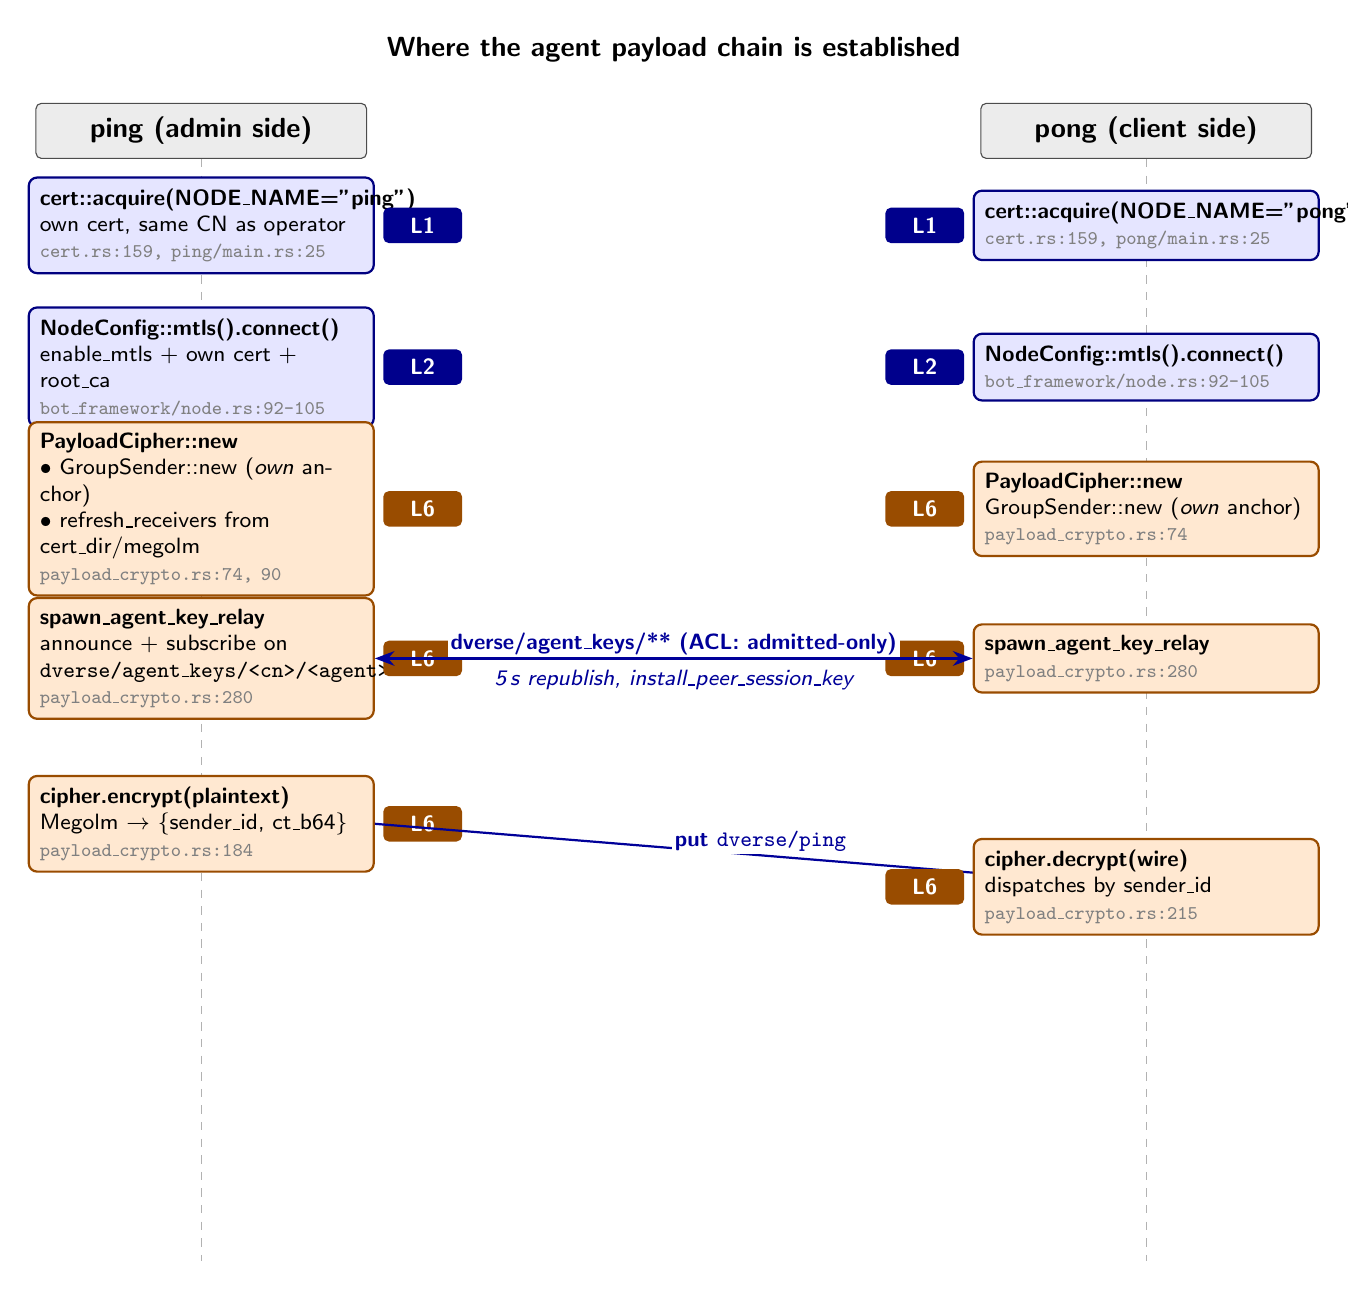
\begin{tikzpicture}[
    actor/.style={
      font=\sffamily\bfseries, align=center,
      draw=black!70, fill=gray!15, rectangle, rounded corners=2pt,
      minimum width=4.2cm, minimum height=0.7cm,
    },
    fabric/.style={
      font=\footnotesize\sffamily, align=left,
      fill=blue!10, draw=blue!50!black, thick,
      rectangle, rounded corners=3pt, inner sep=4pt,
      text width=4.1cm,
    },
    payload/.style={
      font=\footnotesize\sffamily, align=left,
      fill=orange!18, draw=orange!60!black, thick,
      rectangle, rounded corners=3pt, inner sep=4pt,
      text width=4.1cm,
    },
    tag/.style={
      font=\footnotesize\sffamily\bfseries, text=white,
      rectangle, rounded corners=2pt,
      minimum width=1.0cm, minimum height=0.45cm, inner sep=2pt,
    },
    L1/.style={tag, fill=blue!55!black},
    L2/.style={tag, fill=blue!55!black},
    L3/.style={tag, fill=blue!55!black},
    L6/.style={tag, fill=orange!60!black},
    msg/.style={-{Stealth[length=2.5mm]}, thick, blue!60!black},
    relaymsg/.style={{Stealth[length=2.5mm]}-{Stealth[length=2.5mm]}, thick, blue!60!black},
    msglabel/.style={
      font=\footnotesize\sffamily\bfseries, midway, above,
      fill=white, inner sep=1pt,
    },
    life/.style={dashed, gray!60},
]
\node[actor] (P) at (0, 0)  {ping (admin side)};
\node[actor] (Q) at (12, 0) {pong (client side)};

\draw[life] (P.south) -- ++(0,-14);
\draw[life] (Q.south) -- ++(0,-14);

\node[fabric] at (P |- 0,-1.2) (Pacq)
  {\textbf{cert::acquire(NODE\_NAME="ping")}\\own cert, same CN as operator\\\code{cert.rs:159, ping/main.rs:25}};
\node[L1, right=0.1cm of Pacq] {L1};

\node[fabric] at (Q |- 0,-1.2) (Qacq)
  {\textbf{cert::acquire(NODE\_NAME="pong")}\\\code{cert.rs:159, pong/main.rs:25}};
\node[L1, left=0.1cm of Qacq] {L1};

\node[fabric] at (P |- 0,-3.0) (Pconn)
  {\textbf{NodeConfig::mtls().connect()}\\enable\_mtls + own cert + root\_ca\\\code{bot\_framework/node.rs:92-105}};
\node[L2, right=0.1cm of Pconn] {L2};

\node[fabric] at (Q |- 0,-3.0) (Qconn)
  {\textbf{NodeConfig::mtls().connect()}\\\code{bot\_framework/node.rs:92-105}};
\node[L2, left=0.1cm of Qconn] {L2};

\node[payload] at (P |- 0,-4.8) (Pcipher)
  {\textbf{PayloadCipher::new}\\
   $\bullet$ GroupSender::new (\textit{own} anchor)\\
   $\bullet$ refresh\_receivers from cert\_dir/megolm\\
   \code{payload\_crypto.rs:74, 90}};
\node[L6, right=0.1cm of Pcipher] {L6};

\node[payload] at (Q |- 0,-4.8) (Qcipher)
  {\textbf{PayloadCipher::new}\\GroupSender::new (\textit{own} anchor)\\\code{payload\_crypto.rs:74}};
\node[L6, left=0.1cm of Qcipher] {L6};

\node[payload] at (P |- 0,-6.7) (Prelay)
  {\textbf{spawn\_agent\_key\_relay}\\
   announce + subscribe on\\
   \texttt{dverse/agent\_keys/<cn>/<agent>}\\
   \code{payload\_crypto.rs:280}};
\node[L6, right=0.1cm of Prelay] {L6};

\node[payload] at (Q |- 0,-6.7) (Qrelay)
  {\textbf{spawn\_agent\_key\_relay}\\\code{payload\_crypto.rs:280}};
\node[L6, left=0.1cm of Qrelay] {L6};

% Wire relay arrow (bidirectional, ACL-gated)
\draw[relaymsg] (Prelay.east) -- (Qrelay.west)
    node[msglabel, midway] {dverse/agent\_keys/** (ACL: admitted-only)}
    node[font=\footnotesize\sffamily\itshape, midway, below=1mm, fill=white, inner sep=1pt]
      {5\,s republish, install\_peer\_session\_key};

\node[payload] at (P |- 0,-8.8) (Penc)
  {\textbf{cipher.encrypt(plaintext)}\\Megolm $\to$ \{sender\_id, ct\_b64\}\\\code{payload\_crypto.rs:184}};
\node[L6, right=0.1cm of Penc] {L6};

% Encrypted payload from P to Q
\draw[msg] (Penc.east) -- (Q |- 0,-9.6)
    node[msglabel, midway] {put \texttt{dverse/ping}};

\node[payload] at (Q |- 0,-9.6) (Qdec)
  {\textbf{cipher.decrypt(wire)}\\dispatches by sender\_id\\\code{payload\_crypto.rs:215}};
\node[L6, left=0.1cm of Qdec] {L6};

\node[font=\sffamily\bfseries, above=0.4cm of P, xshift=6cm]
    {Where the agent payload chain is established};

\end{tikzpicture}

\end{document}
